\setchapterimage[6cm]{images/004_Headerchapter1.png}
\setchapterpreamble[u]{\margintoc}
\chapter{Mathematical and Physical Background}
\labch{MathAndBackground}

In this chapter I will describe the most common options used, both the 
ones inherited from \Class{scrbook} and the \Class{kao}-specific ones. 
Options passed to the class modifies its default behaviour; beware 
though that some options may lead to unexpected results\ldots

\section{Linear Algebra}

	[Introduction Linear Algebra]
	\subsection{Matrices}
		[Matrices]
	\subsection{Matrix Operation}
		[Determinant]
		[Matrix multiplication]

\section{Reference Coordinate Frames }
\subsection{Cartesian Coordinates}
\subsection{Spherical Coordinates}

\subsection{Earth Centered Inertial - ECI}

\begin{figure}[hb]
	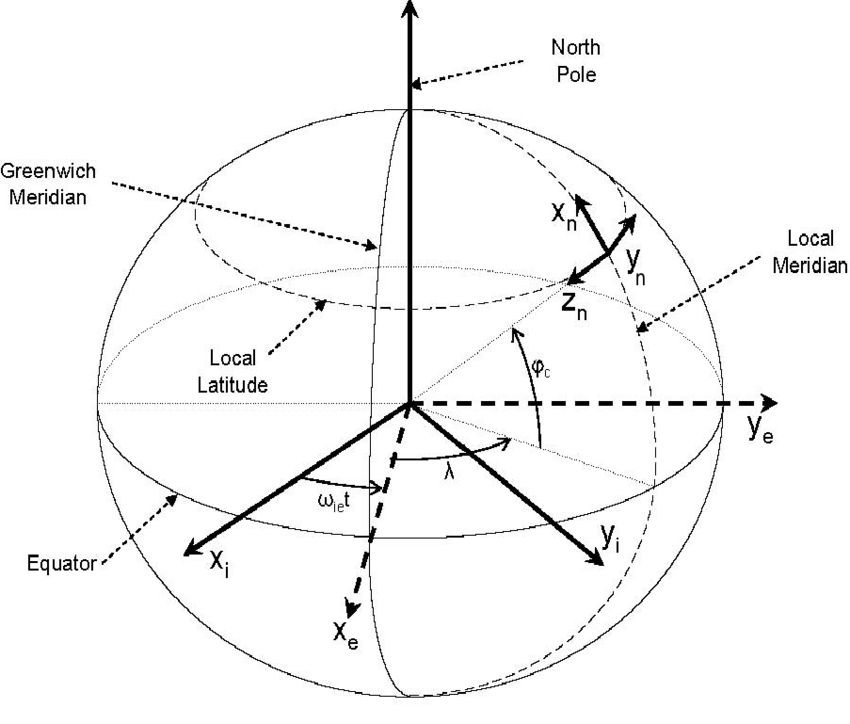
\includegraphics[width=0.45\textwidth]{001_ECI}
	\caption[Earth Centered Intertial]{Earth Centered Intertial. }
	\labfig{fig:eci}
\end{figure}

\subsection{Earth Centered Earth Fixed - ECEF}

\begin{kaobox}[frametitle=Reference Body]
	Note that Earth Centered Inertial as well as Earth Centered Earth Fixed have the strong implication that the reference body is indeed Earth. The basic principle of these coordinate frames however can be applied to any arbitrary planetary body. Since the abbreviation is quite prominent it is common to use ECI and ECEF even if the reference body is not Earth. In the context of this book ECI does not always necessarily refer to Earth.
\end{kaobox}

\subsection{North East Down - NED}
\subsection{Aerodynamic Frame - A}
\subsection{Bodyfixed Frame - B}

\section{Coordinate Frame Transformation}
	\subsection{Spherical to Cartesian Coordinates}
	\subsection{Cartesian to Spherical Coordinates}
	\subsection{ECI to ECEF}
	\subsection{B to NED}
	
	
\section{Equations of Translational Motion}

\section{Equations of Rotational Motion}

\section{External Forces}
	\subsection{Gravitational Forces}
	\subsection{Aerodynamic Forces}
